\documentclass[a4paper, 10pt]{article}
\usepackage[utf8]{inputenc}
\usepackage[spanish]{babel}
\usepackage{hyperref}
\usepackage{tabularx}
\usepackage{inconsolata}
\usepackage{enumitem}
\usepackage{graphicx}

\usepackage{listings}
\usepackage{color}
\usepackage{appendix}
\usepackage{mdframed}
\usepackage{listings}
\usepackage{float}
\usepackage{caption}
\usepackage{subcaption}
\usepackage{subfigure} % subfiguras
\usepackage{multirow}

\newcommand{\cabeceraSI}[2]{
	\begin{center}
	\begin{tabularx}{\textwidth}{|c c|X|X|X|X}
	\hline
	  \multicolumn{2}{|c|}{\multirow{3}{*}{
\includegraphics[scale=0.10]{../uam.png}}} & \multicolumn{4}{c|}{\bfseries Escuela Politécnica Superior}\\
	  & & \multicolumn{4}{c|}{\bfseries Ingeniería Informática}\\
	  & & \multicolumn{4}{c|}{\bfseries Prácticas de Sistemas Informáticos 2}\\
	\hline
	  \multicolumn{1}{|c|}{\textbf{Grupo}} & 2401 & \multicolumn{1}{|c|}{\textbf{Práctica}} & \multicolumn{1}{>{\centering\arraybackslash}X|}{#1} & \multicolumn{1}{>{\bfseries\centering\arraybackslash}X|}{Fecha} & \multicolumn{1}{c|}{#2}\\
	\hline
	  \multicolumn{2}{|c|}{\textbf{Alumno}} & \multicolumn{4}{l|}{Kasner Tourné, Cristina}\\
	\hline
	  \multicolumn{2}{|c|}{\textbf{Alumno}} & \multicolumn{4}{l|}{Guridi Mateos, Guillermo}\\
	\hline
	\end{tabularx}
	\end{center}
}

\definecolor{mygreen}{rgb}{0,0.6,0}
\definecolor{mygray}{rgb}{0.5,0.5,0.5}
\definecolor{mymauve}{rgb}{0.58,0,0.82}

\lstset{ %
	backgroundcolor=\color{white},   % choose the background color; you must add \usepackage{color} or \usepackage{xcolor}
	basicstyle=\footnotesize,        % the size of the fonts that are used for the code
	breakatwhitespace=false,         % sets if automatic breaks should only happen at whitespace
	breaklines=true,                 % sets automatic line breaking
	captionpos=b,                    % sets the caption-position to bottom
	commentstyle=\color{mygreen},    % comment style
	deletekeywords={...},            % if you want to delete keywords from the given language
	escapeinside={\%*}{*)},          % if you want to add LaTeX within your code
	extendedchars=true,              % lets you use non-ASCII characters; for 8-bits encodings only, does not work with UTF-8
	frame=single,                    % adds a frame around the code
	keepspaces=true,                 % keeps spaces in text, useful for keeping indentation of code (possibly needs columns=flexible)
	keywordstyle=\color{blue},       % keyword style
	language=Octave,                 % the language of the code
	morekeywords={*,...},            % if you want to add more keywords to the set
	numbers=left,                    % where to put the line-numbers; possible values are (none, left, right)
	numbersep=5pt,                   % how far the line-numbers are from the code
	numberstyle=\tiny\color{mygray}, % the style that is used for the line-numbers
	rulecolor=\color{black},         % if not set, the frame-color may be changed on line-breaks within not-black text (e.g. comments (green here))
	showspaces=false,                % show spaces everywhere adding particular underscores; it overrides 'showstringspaces'
	showstringspaces=false,          % underline spaces within strings only
	showtabs=false,                  % show tabs within strings adding particular underscores
	stepnumber=2,                    % the step between two line-numbers. If it's 1, each line will be numbered
	stringstyle=\color{mymauve},     % string literal style
	tabsize=2,                       % sets default tabsize to 2 spaces
	title=\lstname                   % show the filename of files included with \lstinputlisting; also try caption instead of title
}

\makeatletter
\def\@seccntformat#1{%
  \expandafter\ifx\csname c@#1\endcsname\c@section\else
  \csname the#1\endcsname\quad
  \fi}
\makeatother

\newcommand{\tabitem}{\vspace{1mm}~~\llap{\textbullet}~~}

\hypersetup{
    colorlinks=true,
    citecolor=black,
    linkcolor=black,
    urlcolor=blue
}

%% Titulo y autores
\title{Sistemas Informáticos 2\\Práctica 2}
\author{Cristina Kasner Tourné\and Guillermo Guridi Mateos}
\date{\today}

%% Documento
\begin{document}

\cabeceraSI{2}{8/04/2015}

\section{Ejercicio 1}
\begin{mdframed} 
Siguiendo todos los pasos anteriores, defina el plan completo de pruebas para realizar las tres 
ejecuciones secuenciales sobre los tres proyectos definidos hasta ahora (P1-base, P1-ws-cli, P1-ejb). 
Adjunte el fichero generado P2.jmx al entregable de la práctica. 
\end{mdframed}
No hemos tenido ningún problema en definir el plan de pruebas tal y como se nos indicaba en el enunciado.

Adjuntamos una imagen con el árbol de resultados.

\begin{figure}[hbtp]
	 	\centering
	 	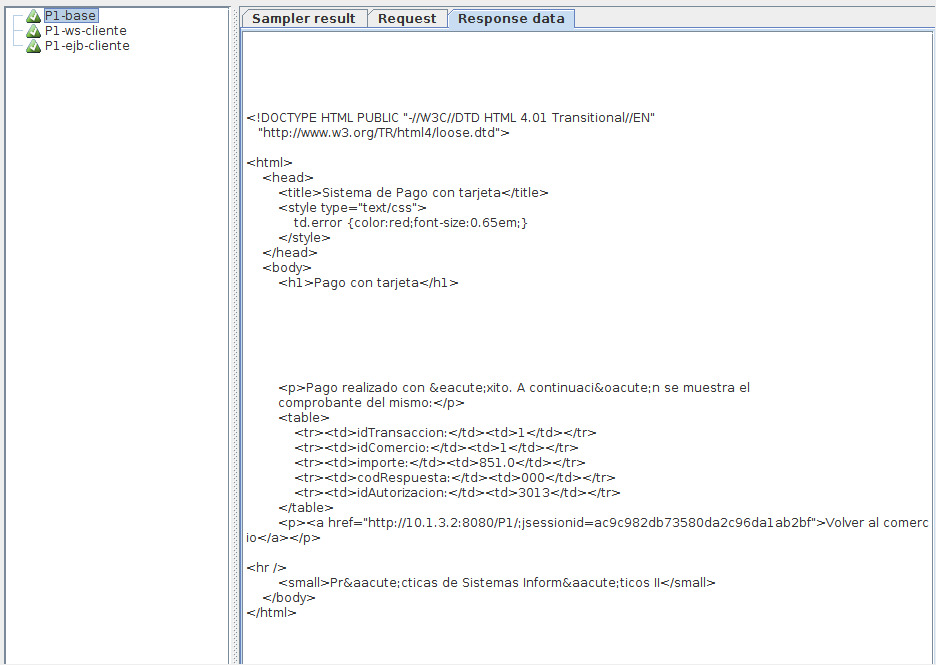
\includegraphics[width=1.1\textwidth]{../../p2/pantallazos/ejemplo_tree_result.png}
	 	\captionÁrbol de resultados}
	 \end{figure}


\section{Ejercicio 2}
\begin{mdframed} 
Preparar los PCs con el esquema descrito. Para ello:
\begin{itemize}
\item Anote en la memoria de prácticas las direcciones IP asignadas a cada PC. 
\item Detenga el servidor de GlassFish de los PCs físicos 
\item Inicie los servidores GlassFish en las máquinas virtuales 
\item Repliegue todas las aplicaciones o pruebas anteriores (P1-base, P1-ws, etc), para limpiar posibles 
versiones incorrectas. 
\item Revise y modifique si es necesario los ficheros build.properties (propiedad “nombre”) de cada 
versión, de modo que todas las versiones tengan como URL de despliegue las anteriormente 
indicadas (P1-base, P1-ws, P1-ejb). 
\item Despliegue las siguientes prácticas: P1-base, P1-ws, P1-ejb, con el siguiente esquema:
	\begin{itemize}
	\item El destino del despliegue en todos los casos será PC2VM con IP 10.X.Y.2 (as.host o 
as.host.client en P1-ws) 

	\item La base de datos en todos ellos será la de PC1VM con IP 10.X.Y.1 (db.host) 

	\item En el caso particular de P1-ws, el servidor SOAP estará en 10.X.Y.1 (variable 
as.host.server)

	\end{itemize}

\end{itemize}
Tras detener / iniciar todos los elementos indicados, anotar la salida del comando “free” así como un 
pantallazo del comando “nmon” (pulsaremos la tecla “m” para obtener el estado de la RAM) tanto en las 
máquinas virtuales como los PCs físicos. Anote sus comentarios en la memoria. 
Pruebe a ejecutar un pago “de calentamiento” por cada uno de los métodos anteriores y verifique que 
funcionan (comprobar resultados en el árbol de resultados). 
\end{mdframed}
 \textbf{Dirección IP asignada al PC 1} : 10.1.3.1 \\
 \textbf{Dirección IP asignada al PC 2} : 10.1.3.2

Tras desplegar y ejecutar free y nmon obtenemos los siguientes resultados:

\begin{figure}[htbp]
\centering
\subfigure[free PC1 antes]{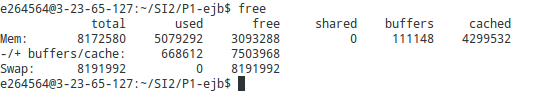
\includegraphics[width=40mm]{../../p2/pantallazos/free_PC_1.png}}
\subfigure[nmon PC1 antes]{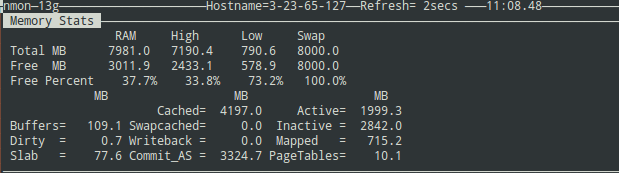
\includegraphics[width=40mm]{../../p2/pantallazos/nmon_pc_1.png}}
\subfigure[free PC1 después]{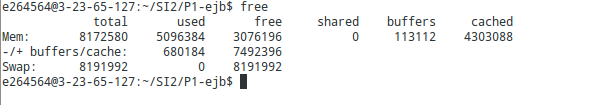
\includegraphics[width=40mm]{../../p2/pantallazos/free_pc1_(glasYpostActiovados).png}}
\subfigure[nmon PC1 después]{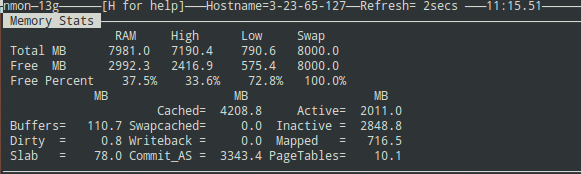
\includegraphics[width=40mm]{../../p2/pantallazos/nmon_pc1_(glasYpostActivados).png}}
\caption{PC 1}
\end{figure}

\begin{figure}[htbp]
\centering
\subfigure[free PC2 antes]{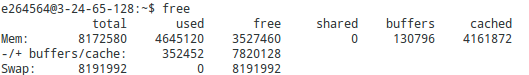
\includegraphics[width=40mm]{../../p2/pantallazos/free_pc_2.png}}
\subfigure[nmon PC2 antes]{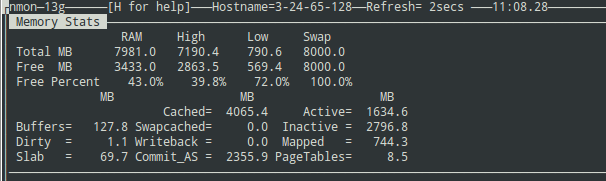
\includegraphics[width=40mm]{../../p2/pantallazos/nmon_pc_2.png}}
\subfigure[free PC2 después]{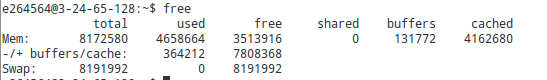
\includegraphics[width=40mm]{../../p2/pantallazos/free_arrancado_PC_2.png}}
\subfigure[nmon PC2 después]{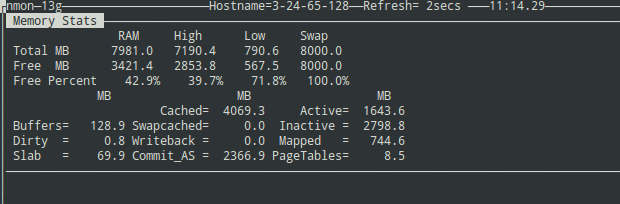
\includegraphics[width=40mm]{../../p2/pantallazos/nmon_arrancado_PC_2.png}}
\caption{PC 2}
\end{figure}

\begin{figure}[htbp]
\centering
\subfigure[free MV1 antes]{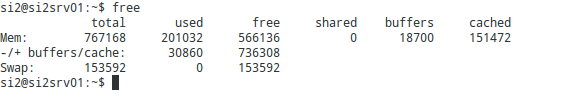
\includegraphics[width=40mm]{../../p2/pantallazos/free_mv_1.png}}
\subfigure[nmon MV1 antes]{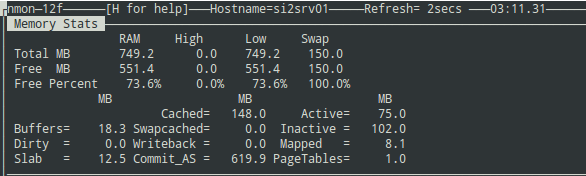
\includegraphics[width=40mm]{../../p2/pantallazos/nmon_mv_1.png}}
\subfigure[free MV1 después]{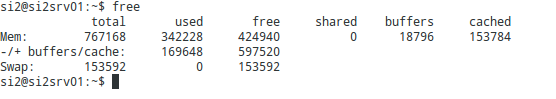
\includegraphics[width=40mm]{../../p2/pantallazos/free_mv1_(freeYpostgresActivados).png}}
\subfigure[nmon MV1 después]{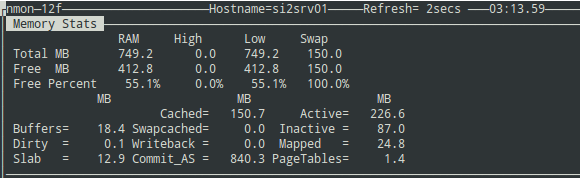
\includegraphics[width=40mm]{../../p2/pantallazos/nmon_mv1_(freeYpostgresActivados).png}}
\caption{máquina virtual 1}
\end{figure}

\begin{figure}[htbp]
\centering
\subfigure[free MV2 antes]{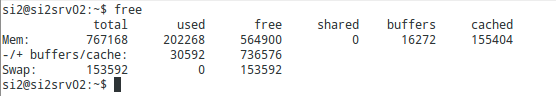
\includegraphics[width=40mm]{../../p2/pantallazos/free_mv_2.png}}
\subfigure[nmon MV2 antes]{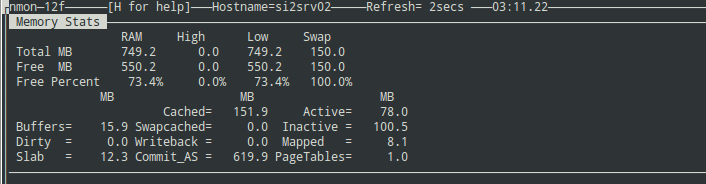
\includegraphics[width=40mm]{../../p2/pantallazos/nmon_mv_2.png}}
\subfigure[free MV2 después]{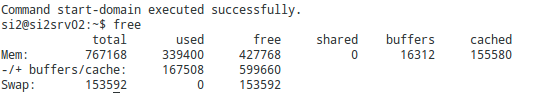
\includegraphics[width=40mm]{../../p2/pantallazos/free_arrancado_mv_2.png}}
\subfigure[nmon MV2 después]{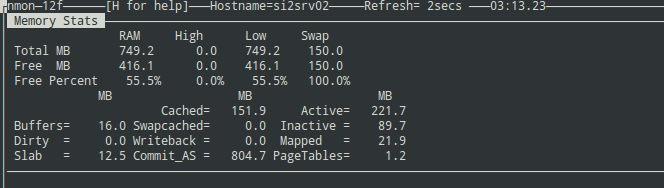
\includegraphics[width=40mm]{../../p2/pantallazos/nmon_arrancado_mv_2.png}}
\caption{máquina virtual 2}
\end{figure}

Podemos observar que al hacer free en los PCs, no hay mucha diferencia en el uso de la memoria estando el glassfish y el postgres arrancados o no. Probablemente esto se deba a que los arrancamos dentro de la maquina virtual que probablemente ya tenga parte de la memoria del sistema virtualizado reservada. Ésto se confirma al comprobar que dentro de las máquinas virtuales si que podemos observar un aumento significativo de la memoria usada (entorno a los 140MB).

Nmon, al usarlo para obtener el mismo tipo de estadísticas nos ofrece las mismas conclusiones.

\end{document}